\chapter{Drawing Primitives}
\section{Drawing a Pixel}
Each pixel is represented in the screeen buffer as a concatenation of byte(8 bits) values for blue, green, red and alpha channels of the pixel colour. Thus the format is B8G8R8A8. The number of bytes required for one row of pixels is called pitch. The screen coordinates originate from top-left. X axis goes towards right and Y axis goes towards down. The pixel rows from top to bottom are stored linearly in the screen buffer.We can actually make an unsigned integer of the blue, green, red and alpha components and store it in one instruction. And that is actually faster way to set pixel. But we chose this for simplicity.

The draw pixel code in C++ is:\\
\lstset{style=cpp}
\begin{lstlisting}

/* Defined earlier in the code:
const int  channels  = 4;
float pitch = width * channels;
*/

inline void SetPixel(int x, int y, int r, int g, int b) {
	unsigned char* dstLoc 
		= pixBuffer + pitch * y 
		+ x * channels;
	*dstLoc++ = b;
	*dstLoc++ = g;
	*dstLoc++ = r;
	*dstLoc = 255;
}
\end{lstlisting}
\clearpage 

\section{Drawing a Line}
For drawing lines we use the DDA algorithm. From the end points of the line the difference in y cordinates and x coordinates are calculated. And further steps of the algorithm are based on comparing those differences. This algorithm uses the fast interpolation trick we saw in chapter section $2.7.1$

The draw line code in C++ is:\\
\lstset{style=cpp}
\begin{lstlisting}
void Canvas::DrawLine(int x0, int y0, int x1, int y1)
{
	float x, y, xIncr, yIncr;
	int steps;
	int dx = x1 - x0;
	int dy = y1 - y0;

	if (abs(dx) > abs(dy)) {
		steps = abs(dx);
	}
	else {
		steps = abs(dy);
	}
	xIncr = dx / static_cast<float>(steps);
	yIncr = dy / static_cast<float>(steps);
	x = x0;
	y = y0;
	for (int i = 0; i < steps; i++)
	{
		int ix = static_cast<int>(x + 0.5f);
		int iy = static_cast<int>(y + 0.5f);
		unsigned char* dstLoc 
			= pixBuffer + pitch * iy + ix * channels;
		*dstLoc++ = primaryColorB;
		*dstLoc++ = primaryColorG;
		*dstLoc++ = primaryColorR;
		*dstLoc = 255;
		x += xIncr;
		y += yIncr;
	}
}
\end{lstlisting}

\clearpage % Ensure the next content starts on a new page

\section{Drawing a Triangle}
To draw a triangle we have three options, viz. draw the vertex pixels, draw the edge lines or draw the filled triangle surface with a rendering method. 
Our triangle rasterizer module for the third case uses a parallelizable method. The method involves finding the bounding box of the triangle's coordinates and, for each point within that bounding box, checking whether it lies inside the triangle. If it does, the vertex attributes are interpolated using its barycentric coordinates: $\alpha$, $\beta$, and $\gamma$. GPUs use this method for rasterization.



\begin{figure}[h!]
\centering
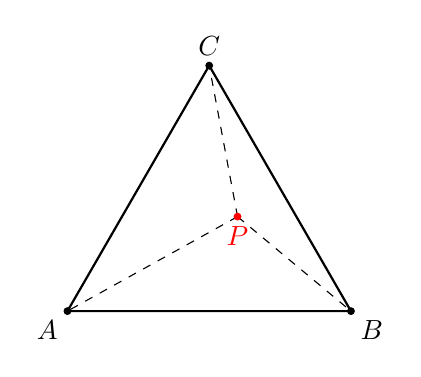
\begin{tikzpicture}[scale=1.2]
  % Define the points
  \coordinate (A) at (0, 0);
  \coordinate (B) at (3, 0);
  \coordinate (C) at (1.5, {3*sqrt(3)/2});  
  \coordinate (P) at (1.8, 1);              

  % Draw the triangle
  \draw[thick] (A) -- (B) -- (C) -- cycle;
  
    \draw[dashed] (P) -- (A);
    \draw[dashed] (P) -- (B);
    \draw[dashed] (P) -- (C);

  \filldraw[red] (P) circle (1pt) node[below] {$P$};

  % Label the triangle vertices
  \filldraw (A) circle (1pt) node[below left] {$A$};
  \filldraw (B) circle (1pt) node[below right] {$B$};
  \filldraw (C) circle (1pt) node[above] {$C$};

\end{tikzpicture}
\caption{Triangle $ABC$ with a candidate point $P$}
\end{figure}


First the signed two times triangle area is calculated from the three vertices using the shoelace formula for a triangle with points A(x1,y1), B(x2, y2) and C(x3, y3). 

\[
2A = \left| 
\begin{array}{ccc}
x_1 & y_1 & 1 \\
x_2 & y_2 & 1 \\
x_3 & y_3 & 1 
\end{array}
\right|
\]

i.e.,
\[
2ABC = x_1(y_2 - y_3) + x_2(y_3 - y_1) + x_3(y_1 - y_2)
\]

For a degenerate triangle this quantity will be zero.\\
And for a backfacing triangle this quantity will be negative.\\
We can omit further processing if those two conditions are met.\\
Then we calculate:
\[
oneOver2ABC = \frac{1}{2ABC}
\]
Now for a point P inside the bounding box of the triangle: \\
We calculate the two times signed area of the triangle formed by the points B, C and P: BCP.\\
If the quantity is less than zero it means P is outside the triangle.\\
We can omit further processing in that case.\\

Then we calculate the two times signed area of the triangle formed by the points C, A and P: CAP.\\
If the quantity is less than zero it means P is outside the triangle.\\
We can omit further processing in that case.\\

alpha = BCP * oneOver2ABC;\\
beta = CAP * oneOver2ABC;\\
gamma = 1 - alpha - beta;\\

We can omit further processing if gamma is less than zero.\\
The quantites alpha, beta and gamma are called barycentric coordinates, they denote the amount of influence of the vertices A, B, C on the point P and so they can be used to interpolate the vertex attributes at P.\\

e.g. P.color = alpha * A.color + beta * B.color + gamma * C.color \\

Here is an example of barycentric interpolation we use in the linear texturing demo in the reference code.
\lstset{style=cpp}
\begin{lstlisting}
void Rasterizer::RasterizeVertices(
	SwrVertex *pv0, 
	SwrVertex *pv1, 
	SwrVertex *pv2) 
{
	vec4f A = pv0->position;
	vec4f B = pv1->position;
	vec4f C = pv2->position;

	texcoord2f tcA = pv0->texcoord;
	texcoord2f tcB = pv1->texcoord;
	texcoord2f tcC = pv2->texcoord;

	const float ABC = EdgeFunction(A, B, C);
	
	if (ABC >= 0) {
		return;
	}

	const float oneOverABC = 1 / ABC;

	int px = 0;
	int py = 0;

	// Get the bounding box of the triangle
	const float minX = MinOfThree(A.x, B.x, C.x);
	const float minY = MinOfThree(A.y, B.y, C.y);
	const float maxX = MaxOfThree(A.x, B.x, C.x);
	const float maxY = MaxOfThree(A.y, B.y, C.y);

	

	// Loop through all the pixels of the bounding box
	for (py = minY; py < maxY; py++) {
		for (px = minX; px < maxX; px++) {
			vec4f P;
			P.x = px;
			P.y = py;
			
			const float BCP = EdgeFunction(B, C, P);
			if (BCP > 0){
				continue;
			}
			const float CAP = EdgeFunction(C, A, P);
			if (CAP > 0){
				continue;
			}

			const float weightA = BCP * oneOverABC;
			const float weightB = CAP * oneOverABC;
			const float weightC = 1 - weightA - weightB;
			if (weightC < 0) {
				continue;
			}

			float interpolatedU = tcA.u * weightA + 
				tcB.u * weightB + 
				tcC.u * weightC;
			float interpolatedV = tcA.v * weightA + 
				tcB.v * weightB + 
				tcC.v * weightC;
			int texureImageX = 
				interpolatedU * oneMinusTextureCanvasWidth;
			int texureImageY = 
				interpolatedV * oneMinusTextureCanvasHeight;
			texureImageY = 
				textureCanvasHeight - texureImageY;

			if (texureImageX < 0) {
				texureImageX = 0;
			}
			else if (texureImageX > oneMinusTextureCanvasWidth){
				texureImageX = oneMinusTextureCanvasWidth;
			}

			if (texureImageY < 0) {
				texureImageY = 0;
			}
			else if (texureImageY > oneMinusTextureCanvasHeight) {
				texureImageY = oneMinusTextureCanvasHeight;
			}

			unsigned char* texel =
				textureCanvasPixels
				+ textureCanvasPitch * texureImageY
				+ texureImageX * 4;
							
			unsigned char* loc =
				canvasPixels
				+ canvasPitch * py
				+ px * 4;
			*loc++ = *texel;
			++texel;
			*loc++ = *texel;
			++texel;
			*loc++ = *texel;
			++texel;
			*loc = *texel;
		}
	}
}
\end{lstlisting}

The perspective correct version of our preceding example is :	\\
P.color = alpha * (A.color / A.w) + beta * (B.color / B.w) + gamma * (C.color / C.w) \\


Here is an example of perspective correct barycentric interpolation, taken from perspective correct texturing demo in the reference code.
Remember each SwrVertex passed to this function has inverse of $w$ is stored as the $w$.
\lstset{style=cpp}
\begin{lstlisting}
void Rasterizer::RasterizeVerticesPerspective(
	SwrVertex *pv0, 
	SwrVertex *pv1, 
	SwrVertex *pv2) 
{
	vec4f A = pv0->position;
	vec4f B = pv1->position;
	vec4f C = pv2->position;

	texcoord2f tcA = pv0->texcoord;
	texcoord2f tcB = pv1->texcoord;
	texcoord2f tcC = pv2->texcoord;

	const float ABC = EdgeFunction(A, B, C);
	
	if (ABC >= 0) {
		return;
	}

	const float oneOverABC = 1 / ABC;

	tcA.u *= A.w;
	tcA.v *= A.w;

	tcB.u *= B.w;
	tcB.v *= B.w;

	tcC.u *= C.w;
	tcC.v *= C.w;


	int px = 0;
	int py = 0;

	// Get the bounding box of the triangle
	const float minX = MinOfThree(A.x, B.x, C.x);
	const float minY = MinOfThree(A.y, B.y, C.y);
	const float maxX = MaxOfThree(A.x, B.x, C.x);
	const float maxY = MaxOfThree(A.y, B.y, C.y);

	// Loop through all the pixels of the bounding box
	for (py = minY; py < maxY; py++) {
		for (px = minX; px < maxX; px++) {
			vec4f P;
			P.x = px;
			P.y = py;

			const float BCP = EdgeFunction(B, C, P);
			if (BCP > 0){
				continue;
			}
			const float CAP = EdgeFunction(C, A, P);
			if (CAP > 0){
				continue;
			}
			const float weightA = BCP * oneOverABC;
			const float weightB = CAP * oneOverABC;
			const float weightC = 1 - weightA - weightB;
			if (weightC < 0) {
				continue;
			}
			float interpolatedOneOverW = 
			(A.w*weightA + B.w*weightB + C.w*weightC);
			float depth = 1 / interpolatedOneOverW;

			float interpolatedU = 
			tcA.u * weightA + tcB.u * weightB + tcC.u * weightC;
			float interpolatedV = 
			tcA.v * weightA + tcB.v * weightB + tcC.v * weightC;
			int texureImageX = 
				interpolatedU  
				* oneMinusTextureCanvasWidth 
				* depth;
			int texureImageY = 
				interpolatedV
				* oneMinusTextureCanvasHeight
				* depth;
			texureImageY = textureCanvasHeight - texureImageY;

			if (texureImageX < 0) {
				texureImageX = 0;
			}
			else if (texureImageX > oneMinusTextureCanvasWidth){
				texureImageX = oneMinusTextureCanvasWidth;
			}

			if (texureImageY < 0) {
				texureImageY = 0;
			}
			else if (texureImageY > oneMinusTextureCanvasHeight) {
				texureImageY = oneMinusTextureCanvasHeight;
			}

			unsigned char* texel =
				textureCanvasPixels
				+ textureCanvasPitch * texureImageY
				+ texureImageX * 4;
							
			unsigned char* loc =
				canvasPixels
				+ canvasPitch * py
				+ px * 4;
			*loc++ = *texel;
			++texel;
			*loc++ = *texel;
			++texel;
			*loc++ = *texel;
			++texel;
			*loc = *texel;
		}
	}
}
\end{lstlisting}
\section{Drawing a Mesh}
Suppose we have a cube. How can we draw it? A cube has 6 quadrilatral faces. So it needs 12 triangle definitions and we just draw each triangle in a loop to render the cube. Similarly we can draw any mesh by iterating the triangles and drawing each of them by our specific rendering pipeline. But how do we load the Wavefront object file? I will tell you the memory format we need. You are requested to code the loader. We load all triangles serially in an std::vector of type  MeshVertex. In the final version, the MeshVertex is composed of position(vec3f), normal(vec3f) and texture coordinate (texcoord2f).

\clearpage